\documentclass[12pt]{article}
\date{May 16, 2020}
\usepackage{pgf-pie}
\usepackage{pgfplots}
\usepackage{pgfplotstable}
\usetikzlibrary{patterns}
\usepackage[section]{placeins}
\usepackage[utf8]{inputenc}

\begin{document}


\clearpage{}
\section{just to delete}

\label{sec:24}


\begin{figure}[h!]
    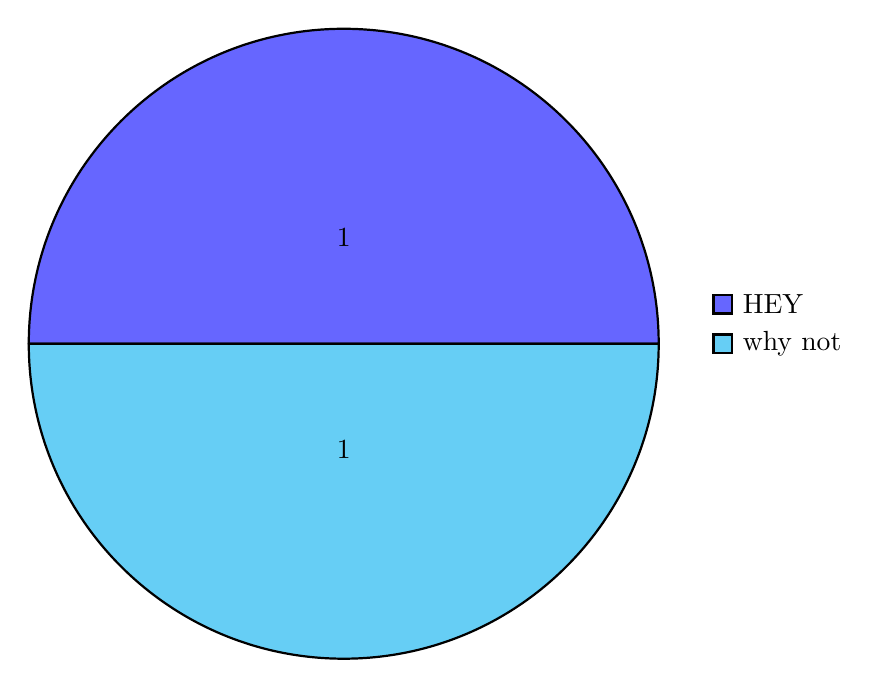
\begin{tikzpicture}
        \pie[radius=4,sum=auto,text=legend]{
            1/HEY,
            1/why not
        }
    \end{tikzpicture}
    \caption{\label{figure:q24-1}Repartition of answers for the question 'just to delete'.}
\end{figure}



\clearpage{}
\section{text mult}

\label{sec:14}


\begin{figure}[h!]
    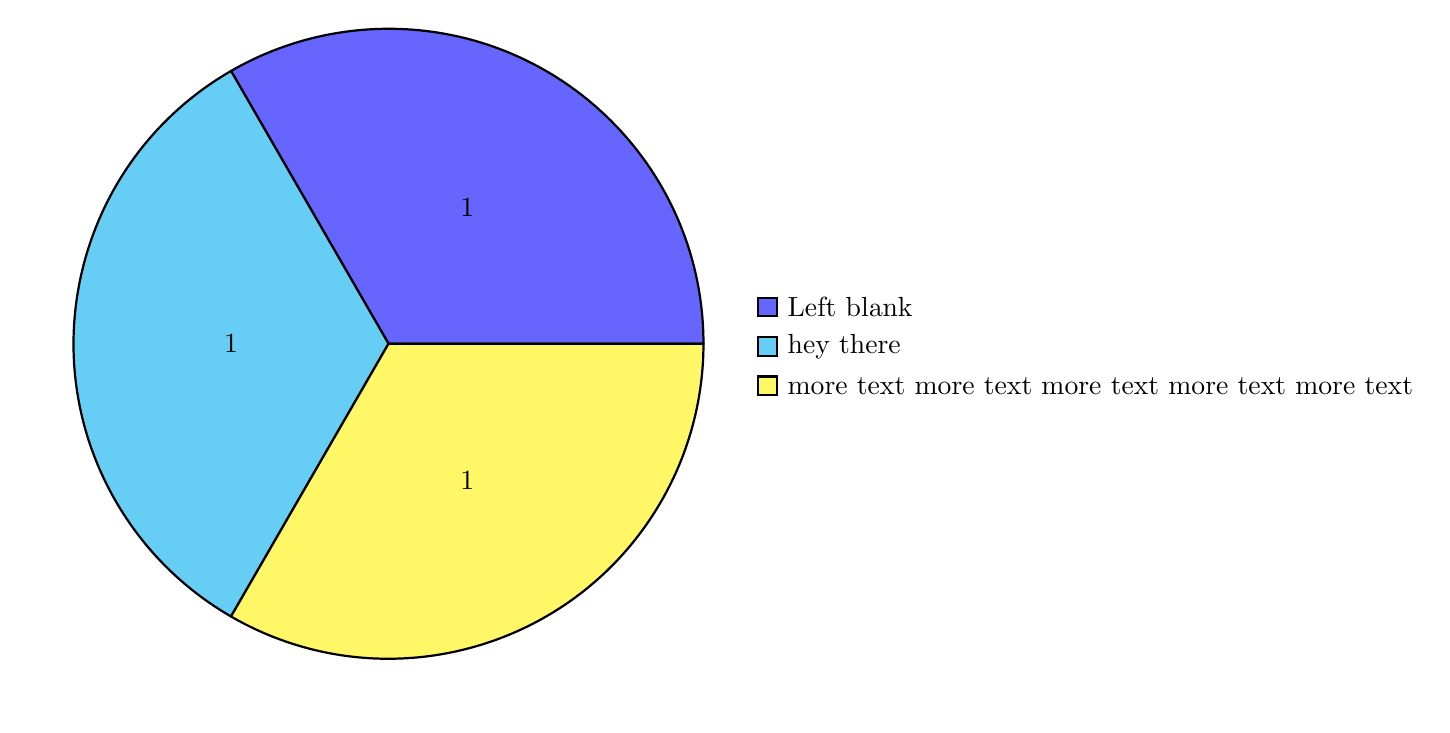
\begin{tikzpicture}
        \pie[radius=4,sum=auto,text=legend]{
            1/Left blank,
            1/hey there,
            1/more text  more text  more text  more text  more text
        }
    \end{tikzpicture}
    \caption{\label{figure:q14-1}Repartition of answers for the question 'text mult'.}
\end{figure}



\clearpage{}
\section{select date}

\label{sec:21}


\begin{figure}[h!]
    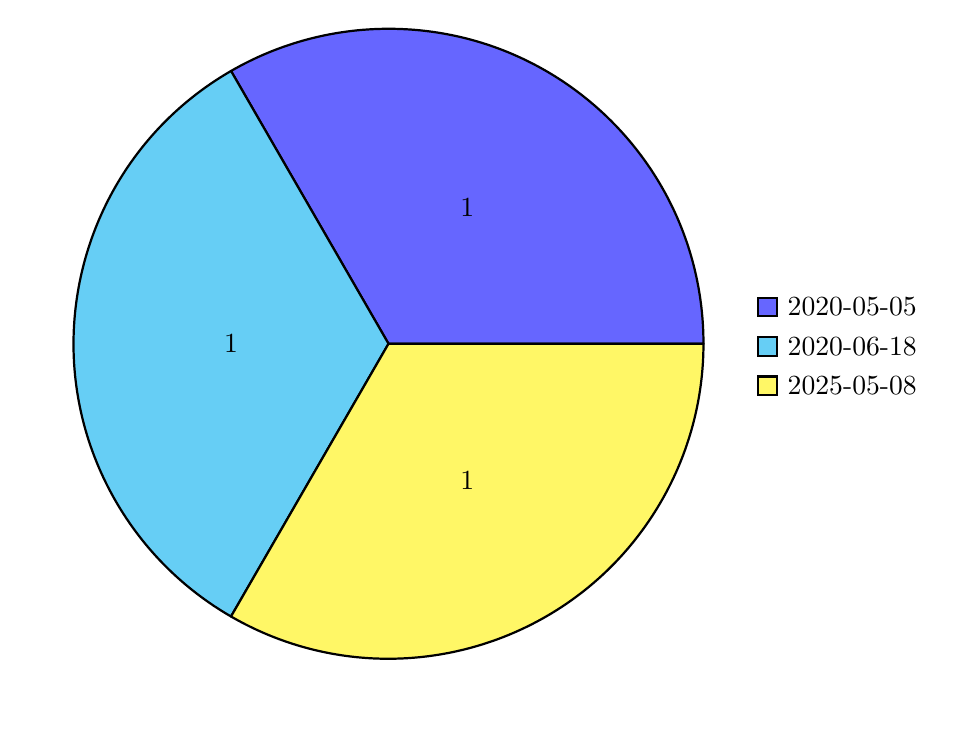
\begin{tikzpicture}
        \pie[radius=4,sum=auto,text=legend]{
            1/2020-05-05,
            1/2020-06-18,
            1/2025-05-08
        }
    \end{tikzpicture}
    \caption{\label{figure:q21-1}Repartition of answers for the question 'select date'.}
\end{figure}



\clearpage{}
\section{how is it going?}

\label{sec:23}


\begin{figure}[h!]
    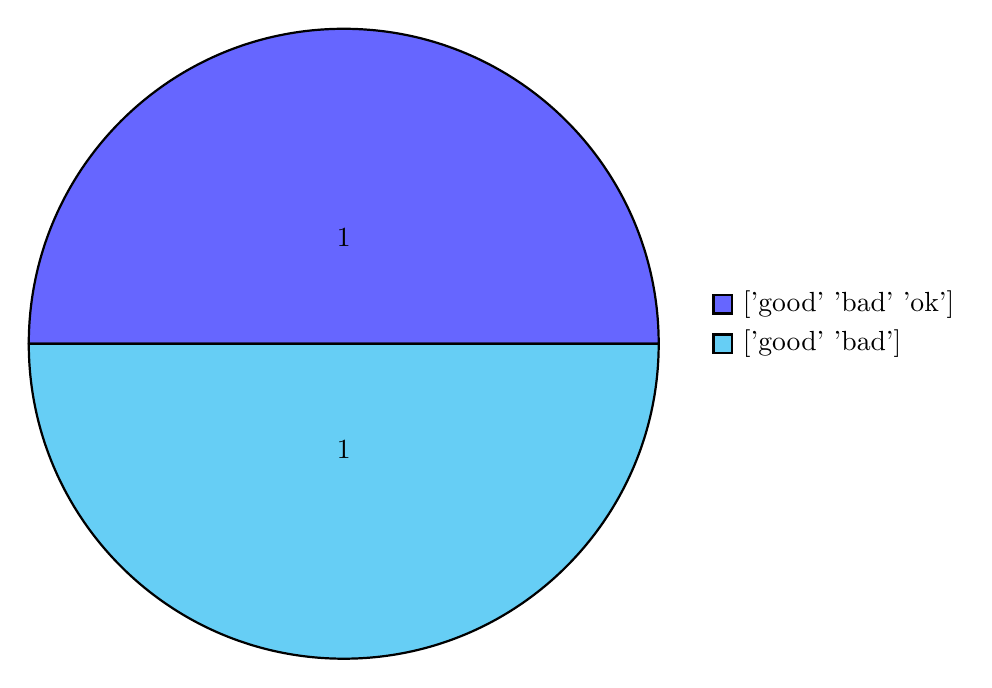
\begin{tikzpicture}
        \pie[radius=4,sum=auto,text=legend]{
            1/['good'  'bad'  'ok'],
            1/['good'  'bad']
        }
    \end{tikzpicture}
    \caption{\label{figure:q23-1}Repartition of answers for the question 'how is it going?'.}
\end{figure}



\clearpage{}
\section{Grade}

\label{sec:29}


\begin{figure}[h!]
    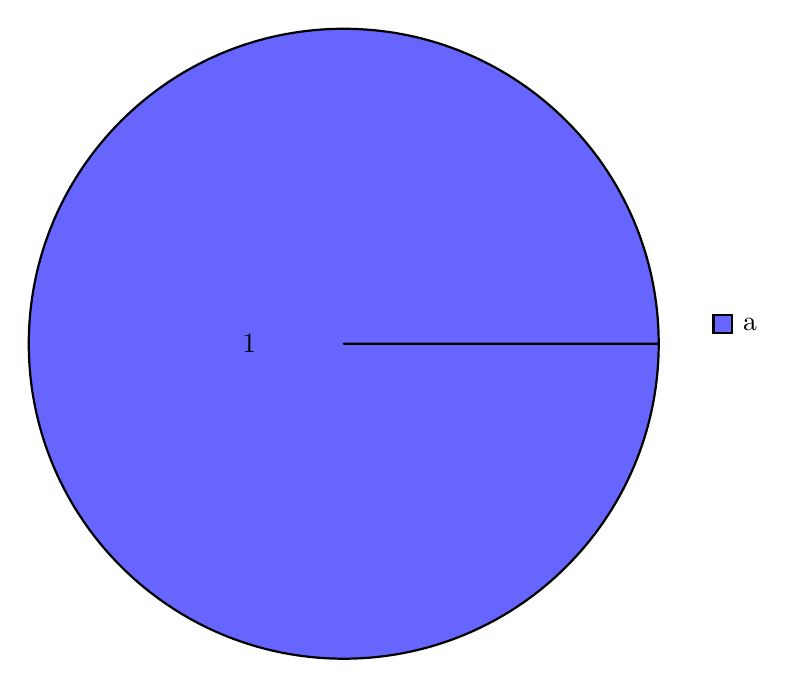
\begin{tikzpicture}
        \pie[radius=4,sum=auto,text=legend]{
            1/a
        }
    \end{tikzpicture}
    \caption{\label{figure:q29-1}Repartition of answers for the question 'Grade'.}
\end{figure}



\clearpage{}
\section{select mult}

\label{sec:18}


\begin{figure}[h!]
    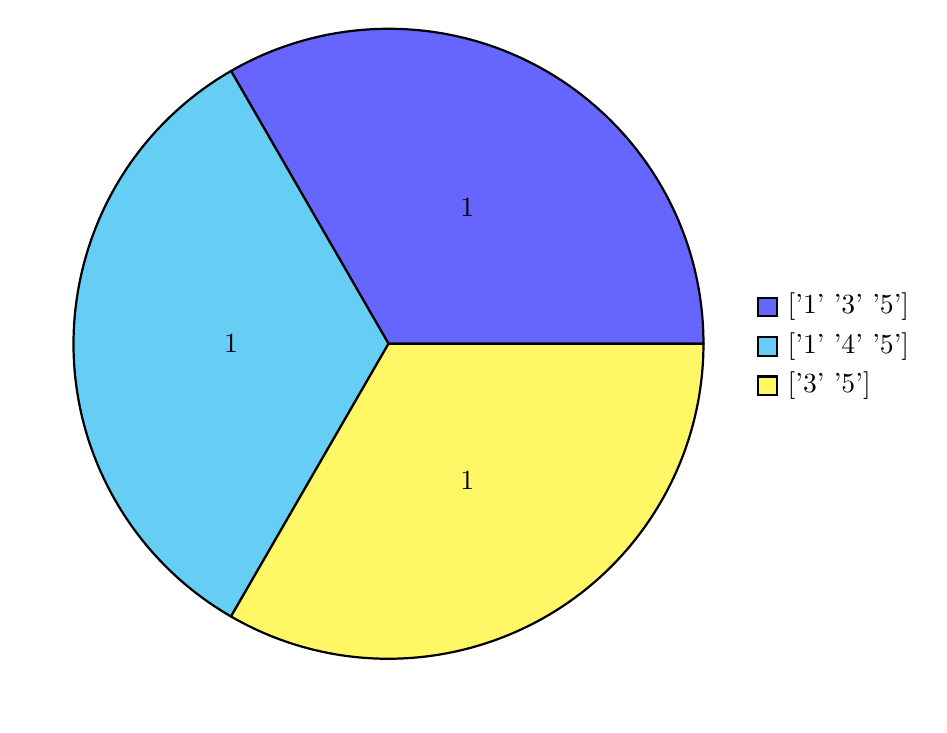
\begin{tikzpicture}
        \pie[radius=4,sum=auto,text=legend]{
            1/['1'  '3'  '5'],
            1/['1'  '4'  '5'],
            1/['3'  '5']
        }
    \end{tikzpicture}
    \caption{\label{figure:q18-1}Repartition of answers for the question 'select mult'.}
\end{figure}



\clearpage{}
\section{short}

\label{sec:15}


\begin{figure}[h!]
    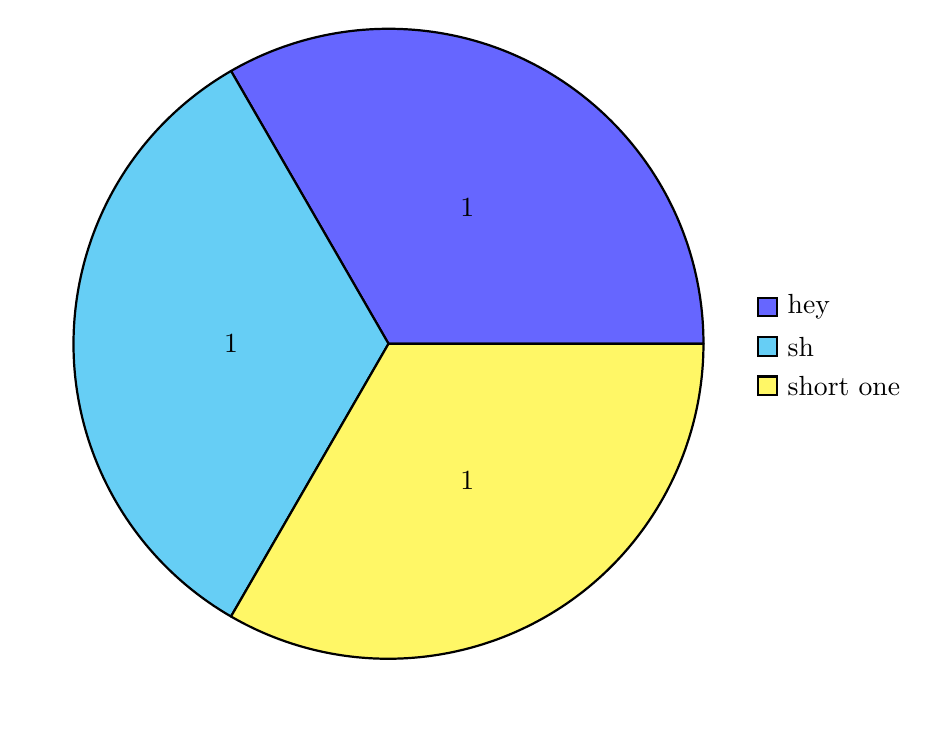
\begin{tikzpicture}
        \pie[radius=4,sum=auto,text=legend]{
            1/hey,
            1/sh,
            1/short one
        }
    \end{tikzpicture}
    \caption{\label{figure:q15-1}Repartition of answers for the question 'short'.}
\end{figure}



\clearpage{}
\section{select}

\label{sec:17}


\begin{figure}[h!]
    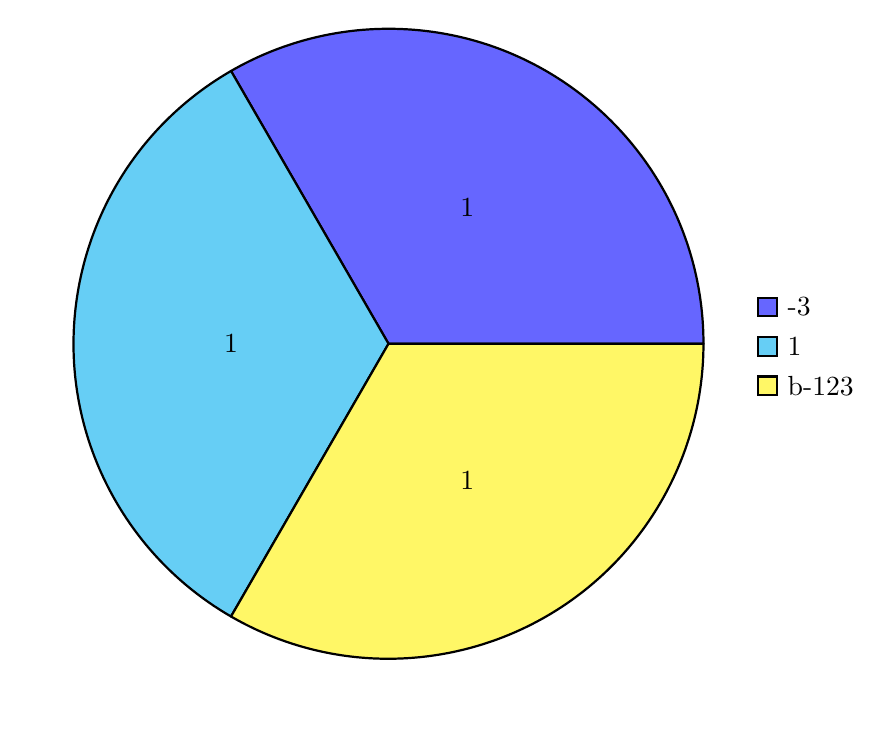
\begin{tikzpicture}
        \pie[radius=4,sum=auto,text=legend]{
            1/-3,
            1/1,
            1/b-123
        }
    \end{tikzpicture}
    \caption{\label{figure:q17-1}Repartition of answers for the question 'select'.}
\end{figure}



\clearpage{}
\section{float}

\label{sec:20}


\begin{figure}[h!]
    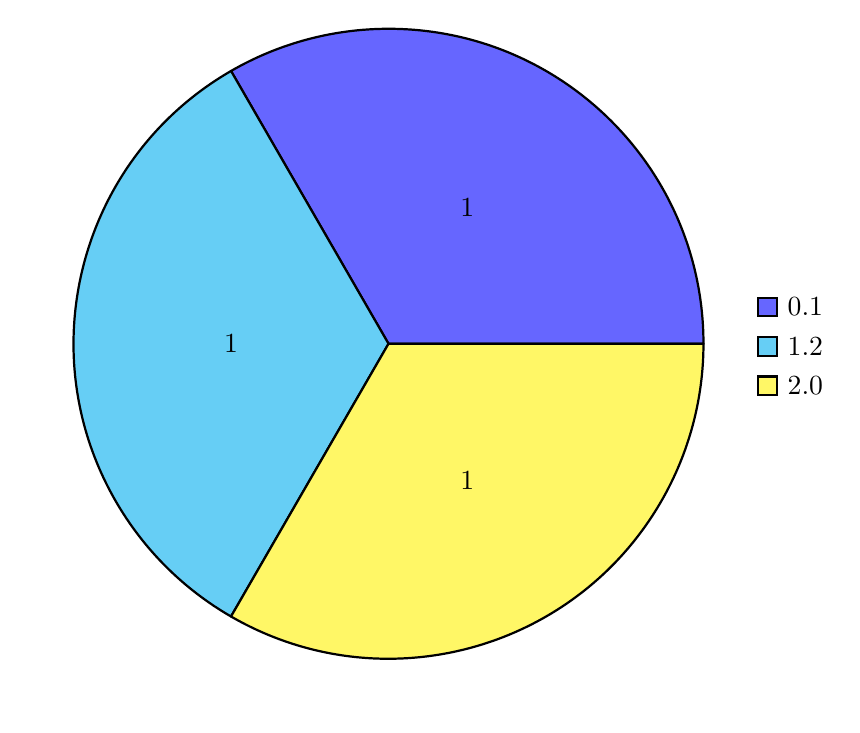
\begin{tikzpicture}
        \pie[radius=4,sum=auto,text=legend]{
            1/0.1,
            1/1.2,
            1/2.0
        }
    \end{tikzpicture}
    \caption{\label{figure:q20-1}Repartition of answers for the question 'float'.}
\end{figure}



\clearpage{}
\section{integer}

\label{sec:19}


\begin{figure}[h!]
    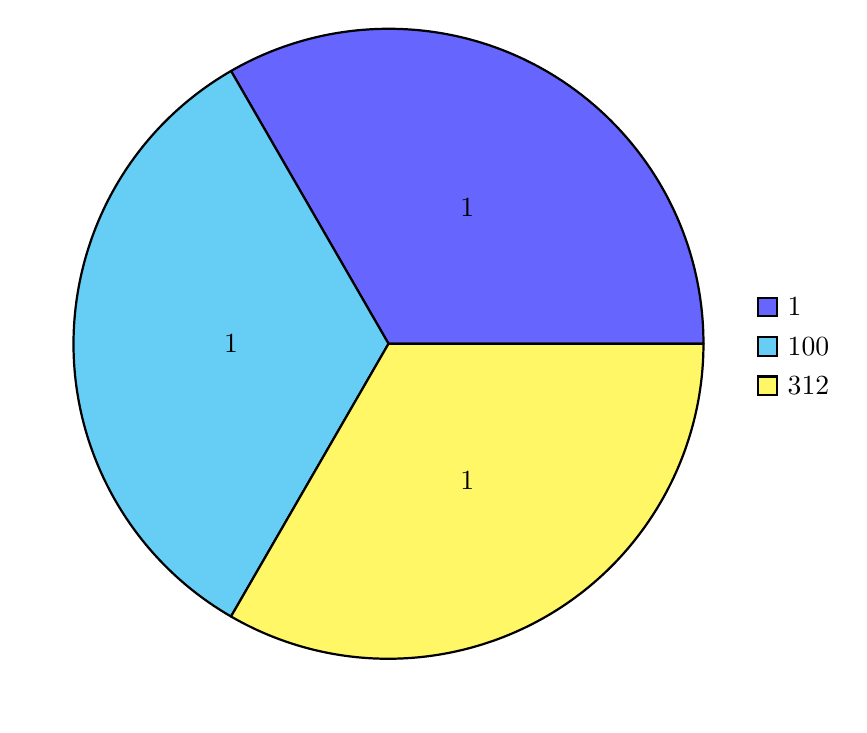
\begin{tikzpicture}
        \pie[radius=4,sum=auto,text=legend]{
            1/1,
            1/100,
            1/312
        }
    \end{tikzpicture}
    \caption{\label{figure:q19-1}Repartition of answers for the question 'integer'.}
\end{figure}



\clearpage{}
\section{radio}

\label{sec:22}


\begin{figure}[h!]
    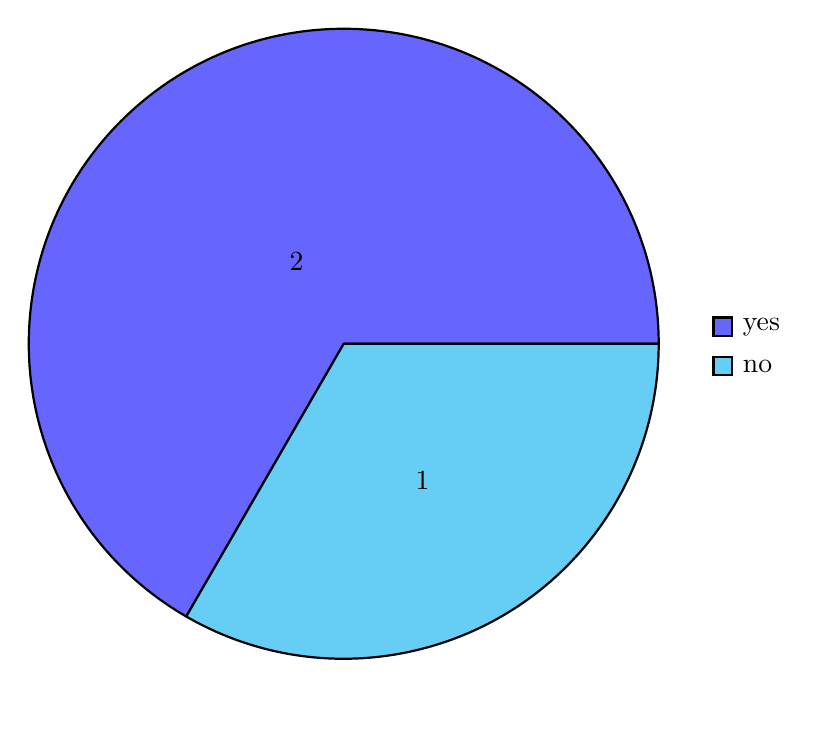
\begin{tikzpicture}
        \pie[radius=4,sum=auto,text=legend]{
            2/yes,
            1/no
        }
    \end{tikzpicture}
    \caption{\label{figure:q22-1}Repartition of answers for the question 'radio'.}
\end{figure}



\end{document}
